\documentclass[14pt,fleqn]{extarticle}
\RequirePackage{prepwell}

\previewoff 

\begin{document} 
\begin{skill}
    \begin{narrow}
    
         De-Morgan's Law 
    \end{narrow}
    
    \reason 
    
    The following two results are called De-Morgan's Law
    \begin{align}
	\left(A\cup B \right)' &= A'\cap B' \\
	\left(A\cap B \right)' &= A'\cup B' 
\end{align}
    
    The results become self-evident when one sees what they look like on a Venn diagram\newline 
    
    In each case, the figure on the right is the \underline{complement} of the figure 
    on the left
    
    \begin{center}
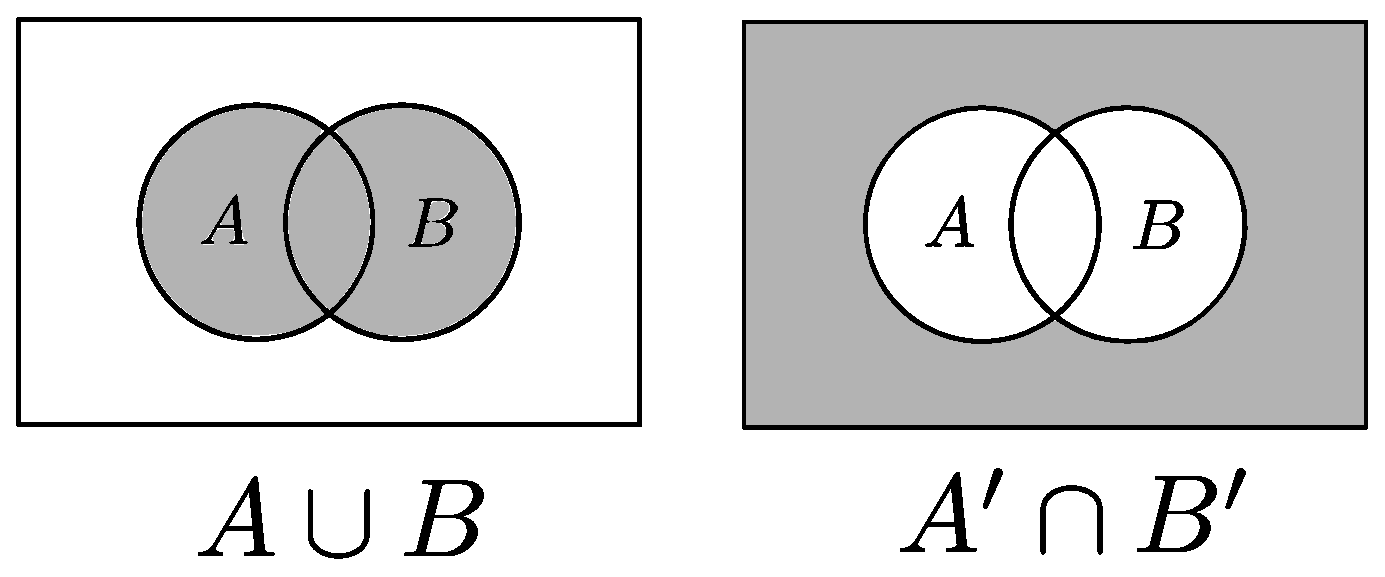
\includegraphics[scale=0.35]{96-A.eps}
\end{center}

\begin{center}
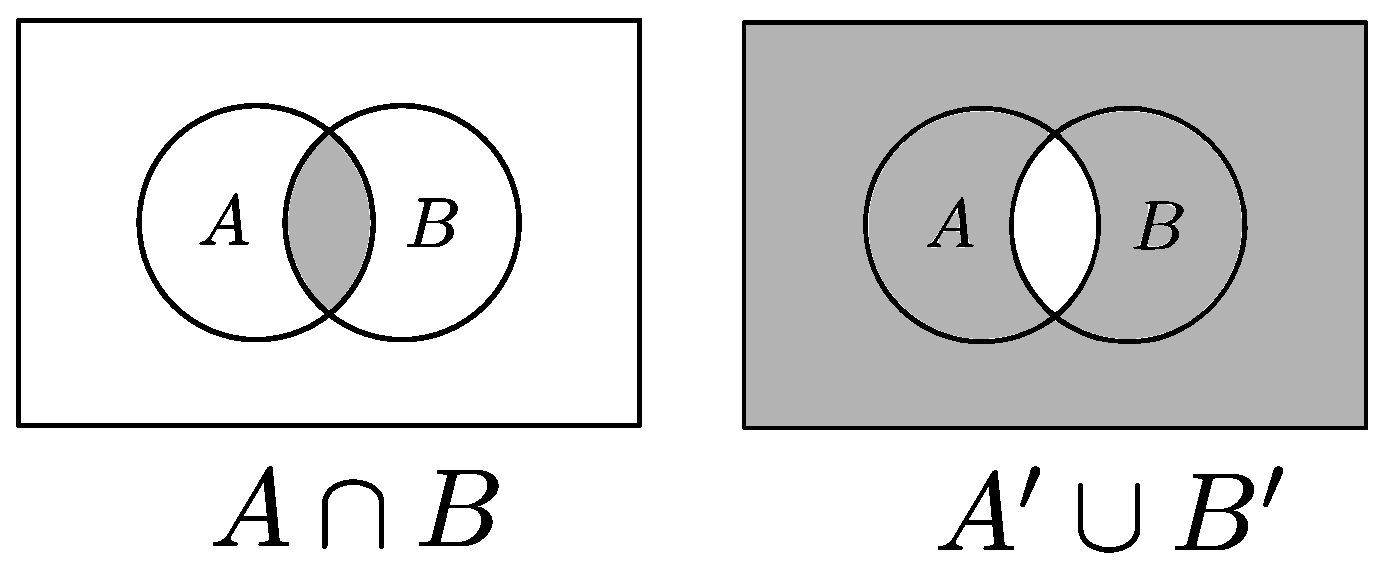
\includegraphics[scale=0.35]{96-B.eps}
\end{center}
\end{skill}
\end{document} 